\subsection{Service}
Most mobile applications use HTTP as a means to communicate with remote services, often through a web interface \cite{maier2010first,falaki2010first}. We will model our service application to that of a stateless web service catering to the subscribers in the local network. The HTTP traffic model in \cite{reyes1999page} provides an open loop traffic model with a long tailed session size distribution, representative of the diversity of mobile the requests. 

Each session is separated in time with a poisson process of $\lambda_{ses}$. Each session produces $N_{req}$ requests, sampled from an inverse Gaussian distribution, where each request is separated in time by log-normal distributed delay $D_{req}$. See Figure \ref{fig:traffic_model}.

\begin{figure*}[tb]
	\centering
	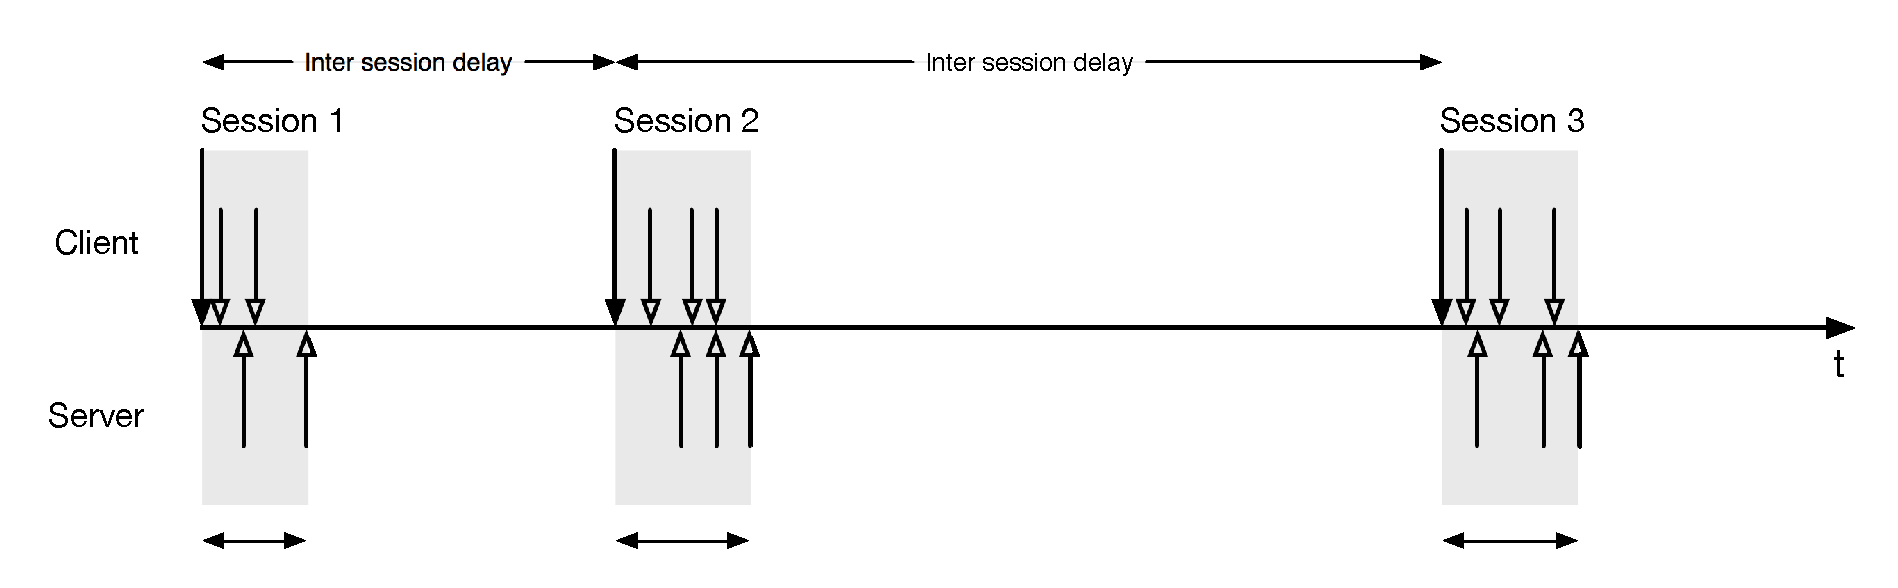
\includegraphics[width=0.8\linewidth]{fig_traffic_model.eps} 
	\caption{Traffic model fundamentals}
	\label{fig:traffic_model}
\end{figure*}

Each service adheres to the same properties, and are only distinguished by the \ac{VM} in which they are running. Additionally, the properties of the service model are independent of \ac{MD} state and mobility mode.

% Even older ; reyes1999page